\documentclass[conference]{IEEEtran}
% \IEEEoverridecommandlockouts
% The preceding line is only needed to identify funding in the first footnote. If that is unneeded, please comment it out.
\usepackage{cite}
\usepackage{amsmath,amssymb,amsfonts}
\usepackage{algorithmic}
\usepackage{graphicx}
\usepackage{textcomp}

\def\BibTeX{{\rm B\kern-.05em{\sc i\kern-.025em b}\kern-.08em
    T\kern-.1667em\lower.7ex\hbox{E}\kern-.125emX}}

\usepackage{url}
\usepackage{comment}
\usepackage{listings}
\usepackage[usenames,dvipsnames,svgnames,table]{xcolor}
\graphicspath{{./figs/}} 
\usepackage{paralist}
\usepackage{hyperref}

\definecolor{dkgreen}{rgb}{0,0.6,0}
\definecolor{mauve}{rgb}{0.58,0,0.82}
\definecolor{light-gray}{gray}{0.88}

\lstdefinestyle{myPromela}
{frame=none,
  basicstyle=\ttfamily,
  language=Promela,
  aboveskip=1mm,
  belowskip=1mm,
  showstringspaces=false,
  columns=flexible,
  numbers=none,
  numberstyle=\tiny\color{gray},
  commentstyle=\color{dkgreen},
  stringstyle=\color{mauve},
  breaklines=false,
  breakatwhitespace=true,
  tabsize=2,
  linewidth=2\linewidth,
  morekeywords={always, eventually, until, implies, ltl}
}

\newcommand{\figref}[1]{Fig.~\ref{#1}}
\newcommand{\secref}[1]{Sec.~\ref{#1}}

\newcommand{\ie}{\textit{i.e.}}
\newcommand{\eg}{\textit{e.g.}}
\newcommand{\etal}{\textit{et al.}}
\newcommand{\etc}{\textit{etc.}}
\newcommand{\adhoc}{\textit{ad hoc}}
\newcommand{\phware}{PHware\textsuperscript{\textregistered}}

\newcommand{\scitesection}[1]{\section{\uppercase{#1}}}

\begin{document}

\title{
  Model Checking Functional Integration of Human Cognition and Machine Reasoning
}

\author{\IEEEauthorblockN{Eric Mercer}
\IEEEauthorblockA{\textit{Brigham Young University}//
Provo UT, USA \\
0000-0002-2264-2958}
\and
\IEEEauthorblockN{Keith Butler}
\IEEEauthorblockA{\textit{BPM+} \\
Seattle WA, USA \\
\url{keith.a.butler@gmail.com}}
\and
\IEEEauthorblockN{Ali Bahrami}
\IEEEauthorblockA{\textit{Bionous LLC} \\
Kirkland WA, USA \\
\url{abahrami@yahoo.com}}
}

\maketitle

\begin{abstract}
    Remote health-care that integrates human and machine intelligence for patient monitoring is an active area of research. These systems must take extra precautions for safety since the patients are not in the direct supervision of medical providers. This paper details the application of model checking to the Bionous \phware\ remote patient monitoring system to prove it preserves patient safety. Patient safety requirements are formalized in a cognitive work problem that is translated to Linear Temporal Logic properties. A cognitive work problem (CWP) is a computationally independent model stating what a system must accomplish. In this example, the system must take action on risk awareness to enhance patient safety, so the CWP defines risk awareness and requisite decisions given the current risk. The \phware\ workflow is translated to Promela to model the asynchronous behaviors of the patient at home, the artificial intelligence in the cloud, and the medical providers. The LTL and Promela models with added behaviors for patient severity are given to the SPIN model checker to prove the system implements the cognitive work problem meaning it acts appropriately in regards to risk awareness. This result is an important contribution to conventional evaluations and contributes to the assurance of patient safety in remote health IT.
\end{abstract}

\begin{IEEEkeywords}
    Model Checking, Business Process Modeling, Model-Based Validation, Model Transformation, Reasoning About Models, Promela, SPIN, Linear Temporal Logic, COVID-19
\end{IEEEkeywords}

\section{Introduction}
There are limited tools for remote objective patient monitoring of diseases where patients may deteriorate quickly. Although tele-health is gaining acceptance for improving accessibility and reducing transmission rates \cite{10.1093/jamia/ocaa048,telehealth,10.1093/jamia/ocaa067}, the remote and asynchronous context of tele-health introduces the risk of a patient's conditions deteriorating before their physicians can be aware and intervene \cite{10.1097/ALN.0000000000003578}. Such risk always exists so the goal is to mitigate and manage that risk to enhance patient safety while in remote care. 

\begin{comment}
  Remote patient monitoring relies on clinicians, health IT, patients-caregivers, and other concurrent actors to each reliably perform various asynchronous tasks to coordinate patient care and safety \cite{remote,Aalam229}. Designing such systems becomes complex quickly because actors are outside the direct control of the system. These distributed and asynchronous characteristics make manual reasoning about functional integration and safety early in the design process very difficult; and yet, early in the design process is exactly the time to clearly establish the utility of the design in fulfilling its intended purpose. 
\end{comment}

This paper introduces a model-based approach for joint human-computer teaming in remote tele-health 
that strives to manage and mitigate some aspects of the inherent risk through formal design verification. The contribution to functional integration is a computationally independent model of the \emph{cognitive work problem} (CWP) that a system must solve \cite{workflowmodel,workcentered,BERRY201615,chi2010}.  A CWP is a complex \emph{object of work} that can be shared by the activities of a distributed cognitive system to transform it from some initial state to the required goal state. The technical neutrality of this object makes it sharable by actors whose performance properties are vastly different; thus, the CWP provides a common basis to represent its state changes that can be performed by a joint team of people and computers. 

The contribution to design verification then re-uses a CWP as a new form of evaluation criterion for model-checking to prove the correctness of the resulting integrated system designs. The capability to integrate human cognition with computer reasoning and then verify the design correctness increases the safety for a wide range of critical systems where human well-being is jeopardized by leaving human-computing teaming to informal approaches \cite{remote,Aalam229}.

This CWP augmented-workflow modeling approach is presented here in a case study of Bionous \phware. \phware is a tele-health application that allows COVID-19 patients to care for themselves at home while remotely monitored by clinicians. It provides a wearable ring or finger-clip to measure vital signs and communicate with a smartphone via Bluetooth. A smartphone application uploads the sensor data to AI cloud services for storage and analysis to increase the accuracy of values assigned to vitals \cite{Altschul2004PredictiveMI,10.2307/2984877,10.5555/1643031.1643047}. A web-based dashboard lets clinicians review vitals, trends, and alerts to prescribe appropriate interventions. 

The paper details the CWP for \phware, developed in conjunction with clinicians and other experts,\footnote{Ann Marie Kimball, an internationally recognized MD epidemiologist in emerging infectious disease, provided medical advice} that defines actionable risk awareness of patients as a finite state diagram with two dimensions: physiological events and actions for appropriate care of the patient. This paper also details the translation of the CWP model into a suite of \emph{Linear Temporal Logic} (LTL) properties that together exactly capture the meaning of the CWP. LTL is a first-order predicate calculus that includes the ability to reason about the temporal ordering of events \cite{10.5555/975331}. Any viable design for tele-health remote monitoring of COVID-19 patients must verify against each LTL property created by the CWP in order to claim it takes appropriate action relative to measured patient risk.

The paper then describes the \phware\ workflow model. The model includes workflows for clinicians, AI cloud services, and patient-caregivers. This paper details how the workflow models for \phware\ are translated into equivalent \emph{Process Meta-language} (Promela) models for the SPIN model checker \cite{spin}. This translation includes behavior models for the environment inputs such as patient vitals. The paper reports the SPIN verification results. All the reported artifacts are available for independent certification \cite{repo}.

The intentions of such a detailed case study are to show the viability of CWP augmented workflow modeling with model checking and to motivate the need for automated reasoning in any design environment. SPIN worked really well in this application in terms of performance and iterative design analysis. The workflows and CWP revisions were easy to verify when posted, and when SPIN found violations, the accompanying counter-examples provided critical insights to the unexpected, and often overlooked, outcomes inherent in asynchronous interactions. These insights were absolutely necessary for those working on the workflows and those working on the CWP to arrive at the presented final forms. The experience of this integrated design process with the model checker makes clear that it is difficult to reliably reason about even simple concurrent systems without a verification tool.

\section{CWP of Actionable Risk Awareness}
\begin{figure*}[t]
  \begin{center}
    \begin{tabular}{c}
      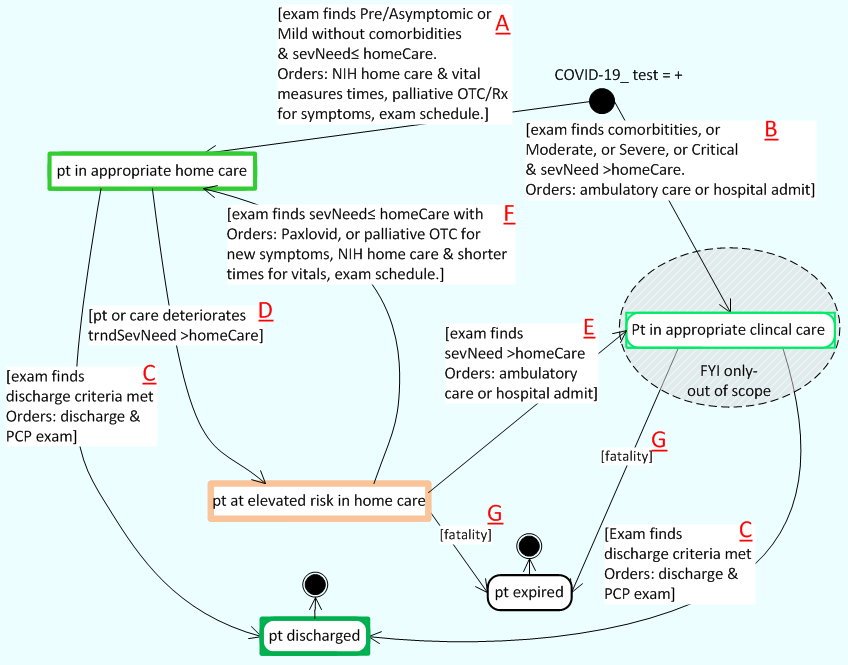
\includegraphics[scale=0.35]{cwp.png}
    \end{tabular}
  \end{center}
\caption{The CWP for remote COVID-19 patient care.}
\label{fig:cwp}
\end{figure*}

\phware is a remote monitoring system that detects and analyzes seven vital signs. Its purpose is to provide clinicians' with timely awareness of their outpatients' conditions and risk during home care, thereby supporting better decisions and enhancing patient safety. This purpose is, however, abstract and intangible. The CWP gives precise meaning to this purpose as a set of transformations on a complex object of work shared by activities in a distributed cognitive system.

To serve as an objective and operational definition of elevated risk due to home care, the work here adapts Medicare’s 4-point severity-of-illness ratings \cite{Hornbrook2005OverviewOD,severity} and the CDC’s Guidance on Home Care \cite{cdc}. The adaptation defines a \emph{Severity Level} less than two as mild, and a \emph{Home Care Capability Level} equal to two as typically appropriate. It then defines \emph{Elevated Outpatient Risk} from home care as either having a \emph{Trending Severity Level} or Severity Level greater than the Home Care Capability Level.

The CWP of actionable risk awareness is developed using these definitions as a finite state diagram, \figref{fig:cwp}, of the relevant care states patients can occupy, their associated risks, and the transition conditions among them. The transition conditions are based on the physician orders (\texttt{orders}), the current severity of the outpatient’s condition assigned by a clinician’s exam (\texttt{sevLvl}), the level of care at the outpatient's residence (\texttt{careCapLvl}), and the trending severity calculated from the remotely monitored longitudinal data as provided by
\phware\ cloud analytics (\texttt{trndSevLvl}). 

In the initial state (top) the patient has tested positive. The arc labeled \textbf{A} occurs when an exam shows symptoms of low severity and a provider orders home care with \phware. Outpatients remain in appropriate home care until either an exam finds discharge criteria met and ordered (\textbf{C}), or the trending severity level is greater than their care capability level (\textbf{D}). In such cases, patients are at an elevated risk in home care. They must not remain at an elevated risk in home care because there is a possible direct path to fatality (\textbf{G}). So a near future exam must either order admission (\textbf{E}), find their risk lower than what the analytics claimed, or make their risk lower with additional prescribed interventions (\textbf{F}). Patients who are admitted to hospital may eventually be discharged back to home care (\textbf{H}) or discharged directly (\textbf{C}). 

The declarative knowledge of the CWP specifies \emph{what} workflows solving the CWP must accomplish without depending on \emph{how} they do it. In this application, the CWP motivates the design, and then when the design is ready, the CWP is the property for formal verification that must be satisfied. Conversely, it is possible to extract a CWP from workflow models in which case the intent is to discover what the system will accomplish. 

The validation of the CWP for \phware\ is an interesting problem that is outside the scope of this paper but merits some discussion. Doctors reviewed the CWP using it as a kind of story-board whose rules at each arc are verified as appropriate care. One review noted that the CWP does not distinguish among causes of fatalities but concluded that any patient trending towards fatality must receive life-saving care regardless of co-morbidities, and so no change was required. The SPIN verification also served to validate the CWP and an example of that is given in \secref{sec:results}.



\section{CWP Translation to LTL}
The CWP in \figref{fig:cwp} is a finite state machine, which is a recognized standard that widely used in software development making it very suitable for specifications. The same is not true for LTL, but LTL, or some variant, is the common language for model checking properties. As such, the CWP is translated to a set of system properties about the whole of the CWP and a set of state properties about each individual state of the CWP. Together these exactly define the meaning of the CWP in LTL. The properties themselves are purposed to be simple and small to mitigate the complexity cost of model checking, since it correlates roughly with property size, and to make it easy to reason about the meaning of each individual property and the collective meaning of all the properties. 

The properties are expressed over atomic propositions with one atomic proposition for each state of the CWP. Each atomic proposition is computed from the conditions on its incoming ($I$) and outgoing ($O$) transitions on the associated CWP state as $(\bigwedge_{i \in I}\ i) \wedge \neg(\bigvee_{o \in O}\ o)$. So an object state resides in a given CWP state if all the conditions on the incoming transitions of the CWP hold for the object state and none of the conditions on the outgoing transitions of the CWP hold for the object state.

Consider the \emph{Pt in appropriate home care} state in \figref{fig:cwp}. The conjunction of the incoming transitions require
%
\[
\begin{array}{l}
  \mathtt{sevLvl} < 2\ \wedge\ \\
  \mathtt{orders} = (\mathtt{homeCare}\ \mathrm{with}\ \mathtt{remote}\ \vee \\
                    \mathtt{more} \vee \mathtt{adjustedRx})
\end{array}
\]
%
The negated disjunction of the outgoing transitions require
%
\[
  \mathtt{orders} \neq \mathtt{discharge} \wedge \mathtt{tndSevLvl} \le \mathtt{careCapLvl}
\]
%
\noindent These together must by true of the object state for the patient to reside in the \emph{Pt in appropriate home care} state. The term \texttt{ptInAppropriateHomeCareState} is the atomic proposition for the state. Such an atomic proposition is defined similarly for each of the other states in \figref{fig:cwp}.

\subsection{System Properties}
There are two system requirements for any CWP. The first is that no object state exists that is not covered by one of the states in the CWP (e.g., the CWP states are universally inclusive); and the second is that the goal states exists. The first property is given by the following atomic proposition and LTL formula.
%
{\small
\begin{lstlisting}[style=myPromela]
#define inAState  InitState || HospitalState 
 || ptInAppropriateHomeCareState 
 || ptInElevatedRiskHomeCareState
 || ptDischargedState || ptExpiredState
ltl alwayInAState {(always (inAState))}
\end{lstlisting}
}
%
\noindent The property is an invariant over the disjunction of CWP states. The object state must \emph{always} be in some known CWP state throughout the entirety of the workflow model execution. The meaning of \emph{always} in LTL is that the \texttt{inAState} expression is true in every state along every path of the workflow model.

The second system level property looks for executions ending in the goal states. The goal states for the CWP in \figref{fig:cwp} have no outgoing transitions and are the \emph{Pt expired} and \emph{Pt discharged} states.
%
{\small
\begin{lstlisting}[style=myPromela]
#define fair (((eventually 
  (   ptDischargedState 
   || ptExpiredState))))
ltl fairPathExists {(always (! fair))}
\end{lstlisting}
}
%
\noindent Here \texttt{fair} is an eventuality that should exist in the workflow. The meaning of \emph{eventually} is that at some point in the future of the path currently being considered, there exists a state, where the expression \texttt{(ptDischargedState || ptExpiredState)} is true. The property to verify is expressed as an invariant using the \emph{always} operator. This invariant \emph{should not hold} in the workflow model (e.g., it should result in a verification error). 

The very nature of LTL makes existential properties awkward to express in that they are accomplished by writing a property that should not hold. The counter-example to the property showing where it does hold is a \emph{witness} to the existential property. Claiming that the eventuality \texttt{fair} never holds in any state in any path of the workflow means that if it does hold somewhere (e.g., exists), then the model checker will find a witness attesting as much. Anytime a property is used on the left-hand side of an implication, then such an existential property should be verified. More on this requirement later.

\begin{comment}
The term \emph{fair} is a reference to the over-approximating nature of the workflow model. Indeed, in considering the workflow in \figref{fig:bpmn}, it is possible that a patient is never discharged or that the patient never expires. Such a behavior is \emph{not fair} because it is not emblematic of the real world---patients eventually are discharged or expire. As such, the property proves the existence of paths in the workflow that end in the goal states, and this same property is used later to restrict verification to only those paths that end in one of goal states thereby excluding from consideration, in verification, any infinite workflow behaviors where the patient never recovers or expires.
\end{comment}

\subsection{Required State Properties}
There are three properties checked at each state. The first is that the state exists somewhere in the workflow model; the second is that the object is never in the state at the same time it is in another state; and the third is that only transitions allowed by the CWP are taken. These are shown by example with the \emph{Pt in appropriate home care state}.

The first state property proves the existence of the state somewhere in the workflow model.
%
{\small
\begin{lstlisting}[style=myPromela]
ltl ptInAppropriateHomeCareExists 
{(fair implies 
  (always (! ptInAppropriateHomeCareState)))}
\end{lstlisting}
}
%
\noindent The property should fail verification because the counter-example is the witness that it does exist. Notice the use of \texttt{fair} in the implication in the property. If the left side of the implication is false, meaning that the workflow path being considered is not fair (e.g., the patient never recovers nor expires), then the implication is satisfied by definition because it is vacuously true; however, if it is a fair path, then that path is checked for the existence of the state. An existential property is added to every implication to avoid vacuity.

The second state property proves the state is mutually exclusive to the other states in the CWP.
%
{\small
\begin{lstlisting}[style=myPromela]
ltl ptInAppropriateHomeCareMutex {
  (always 
    (ptInAppropriateHomeCareState implies ((
         (! InitState) 
      && (! HospitalState) 
      && ptInAppropriateHomeCareState 
      && (! ptInElevatedRiskHomeCareState) 
      && (! ptDischargedState) 
      && (! ptExpiredState)))))}
\end{lstlisting}
}
%
\noindent When the system is in the \emph{Pt in appropriate home care state} state, it cannot be in any of the other CWP states. 

The third state property proves that only transitions allowed by the CWP are implemented by the workflow.
%
{\small
\begin{lstlisting}[style=myPromela]
ltl ptInAppropriateHomeCareEdges {
  (fair implies (always 
    (ptInAppropriateHomeCareState implies (
      ptInAppropriateHomeCareState until (
            ptInElevatedRiskHomeCareState
        ||  ptDischargedState)))))}
\end{lstlisting}
}
%
\noindent Here the workflow stays in the indicated state \emph{until} it transitions to one of the two successor states allowed by the CWP.  The \emph{until} operator requires that at least one of the states on the right of the operator exists somewhere in the future of the path being considered. Those states are either \emph{Pt at elevated risk in home care} or \emph{Pt discharged}. The \emph{Pt in appropriate home care state} must be found in every state up to the point where the first state on the right of the operator is found. 

There are twenty total properties at the end of translation: the two system properties with the three properties for each state in the CWP. These must all hold to verify.


\section{Workflow for Functional Integration}
\begin{figure*}
  \begin{center}
    \begin{tabular}{c}
      \includegraphics[width=6.98in]{bpmn.png}
    \end{tabular}
  \end{center}
\caption{The \href{https://github.com/ericmercer/SPIN-bpmn-cwp-verification-paper/blob/main/16-Feb-2022-BPMN-resources.png}{workflow model} for the \phware\ system.}
\label{fig:bpmn}
\end{figure*}

\figref{fig:bpmn} shows the PHware system design was developed in the \emph{Business Process Model Notation} (BPMN) \cite{BPMN} \cite{BPMNSpecification} using the The MATH tool-suite \cite{workflowmodel}.
The colored lanes represent the activities of clinicians, AI cloud services, and patient/care-givers.
The benefits of adapting BPMN to health care informatics are demonstrated by the recent \emph{BPM+} project of the Object Management Group.\footnote{Many thanks to Stephen White for reviewing the workflow and clarifying aspects of the BPMN semantics.}

Our method for functional integration was adapted from concurrent design engineering in aerospace, where specific tracks for multiple design disciplines coordinate their work by referencing a common physical design artifact \cite{10.1007/978-1-4471-1538-0_9}.
The technology-neutral CWP is pivotal for integrating cognitive work, and extends the notion of higher-order unification \cite{10.1007/3-540-45685-6_2} to joint, human-computer teaming. The CWP served as the common artifact for concurrent engineering, and the colored lanes as tracks to design the coordinated activity of clinicians, AI cloud services, and patient-caregivers. %to transform the CWP to establish and maintain \emph{actionable risk awareness}.

\figref{fig:bpmn} starts in the upper left of the green clinicians' workflow.
Positive test results get exams in task-01. The bold letters in the lanes correlate to transitions of the CWP in \figref{fig:cwp}.
If exams find comorbidities, or moderate, or severe the flow goes to task-03 where the patients get ambulatory care or hospital admission (\textbf{B}).
Severity needs that can be met by home care flow to task-02 that orders home care (\textbf{A}/\textbf{F}).
Discharge criteria include additional tests with negative results following a recovery period (\textbf{C}).

The tan workflow of patient/caregiver begins with task-04, then task-05 repeats recording vitals at ordered times until an exam results in patient discharge, or patient get another exam, or expire (\textbf{G}). 
The raw vitals data are transmitted by smartphone app to AI cloud services in the middle, metallic lane. The Personal Data Analyzer uses machine-learned algorithms in task-06 to assign numerical vital sign values to the sensor data, then analyzes the longitudinal trends of vital signs.
A packet of values and trends is sent immediately to the upper-right of the clinicians' green workflow. An elevated risk alert is added if any combination of current/trending values exceed home care capability.

Alerts skip any routine delay for clinicians' attention in task-07a. A specialized dashboard used in tasks-07a/b provides risk awareness of each patient.
The workflow and user interface were designed to preserve clinicians' ultimate decision authority.
They can quickly access AI reasoning, confirm the current/trending severity justifies the alert, or dismiss it.
If alerts are confirmed task-08a orders urgent teleheath exams that can be set up quickly with real-time vital signs.
Urgent exams may give orders for ambulatory care or hospital admission (\textbf{E}).

Clinicians may also decide trends can be controlled by adjusting orders for more frequent vitals, or oral medication for new discomfort, or \emph{Paxlovid}\textsuperscript{\texttrademark}\ to reduce progression. (\textbf{F}).
When multiple patients have alerts, providers must prioritize them based on familiarity and professional judgement.

If alerts are dismissed routine exams still may be ready to begin soon, or routine exams may be due for scheduling in task-08b. 
For non-alerts, providers review vitals in task 07b when time permits. They may order routine exams that are due to be scheduled by task 08b.
Alternatively, if clinical judgment deems appropriate, providers may order urgent exams in task 08a.
The far right decision gate \textbf{Xor11} is where all exam times are managed.
All approaching exams, whether urgent or scheduled, flow back to task-01, then are held when all participants arrive.

\section{BPMN Translation to Promela}
\label{sec:bpmn}
The top green clinicians lane and the bottom salmon colored patient-caregiver lane in the workflow model in \figref{fig:bpmn} are directly modeled with a \emph{process} in Promela while the middle lane for the AI cloud server is implicitly modeled by the communication between the two processes. In other words, there is a non-deterministic choice in the patient/caregiver process at task 05 to set a value for \texttt{trndSvl}, and the Promela semantics, by definition, deliver that value at some point to the clinician process. Adding the extra process for the AI cloud server does not affect, or change, this explained basic behavior; it only serves to add non-necessary complexity.

The basic structure the for the clinicians and the patient-caregiver processes have the following structure.
%
{\small
\begin{lstlisting}[style=myPromela]
active proctype name() {
  /* Add tokens to initial elements */
  do
  :: (hasToken(element_0)) ->
    /* Model for element_0 activation */
  :: hasToken(element_1) ->
    /* Model for element_1 activation */
 
    /* activations for other elements */
    
  :: hasToken(element_n) ->
    /* Model for element_n activation */
  od
}
\end{lstlisting}
}
%
\noindent The Promela do-statement repeats infinitely often with each \emph{::} being a possible choice for the current iteration of the loop. The expression at each \emph{::} is a condition determining when a choice is available or not in the current iteration. In this way, the model checker must consider all combinations of active choices at each iteration of the loop, and thereby, resolve any and all interleaving of concurrent actions that may take place in the workflow associated with the process. The \texttt{(hasToken(element\_0))} expression has basis in the BPMN semantics.

The distributed and asynchronous BPMN semantics, as described in the standard, flow tokens through the workflow model to control activation of elements. As such, every visual construct defines activation conditions based on arrived tokens. Each element also defines what happens at activation in terms of consuming incoming tokens and generating outgoing tokens. The Promela model of the workflow follows these token based semantics. Each choice in the do-statement is associated with an element of the workflow. And the choice is active if the element meets its activation conditions based on tokens at its incoming edges.

For example, the diamond shaped gates in the workflow model are all exclusive-or gates as indicated by the small 'x' in the bottom corner. Here is the Promela implementation of the \texttt{Xor5} gate on the left of the clinician lane.
%
{\small
\begin{lstlisting}[style=myPromela]
:: hasToken(clinicianXor5) ->
  atomic {
    consumeToken(clinicianXor5)
    if
    :: isRequiresHospital(sevLvl) ->
      putToken(clinicianTask03)
    :: (!isRequiresHospital(sevLvl) && 
         isDischarge(orders)) ->
      putToken(clinicianEnd61)
    :: else ->
      putToken(clinicianTask02)
    fi
  }
\end{lstlisting}
}
% 
\noindent The \emph{::} denotes that the \texttt{Xor5 severity} gate is one of the several choices that may be available at any iteration of the do-loop in the clinicians process. The atomic-statement means that all the enclosed statements happen in a single-step of the model and cannot be sub-divided by any other interleaving action from another process.

The \texttt{clinicianXor5} is a global variable to represent the presence or absence of a token on the incoming edge of the gate: \texttt{bit clinicianXor5 = 0}. The \texttt{hasToken}, \texttt{consumeToken}, and \texttt{putToken} macros have their implied intuitive meanings. The if-statement outputs the token on the appropriate edge depending on the \texttt{sevLvl} as indicated by the BPMN model in \figref{fig:bpmn}. 

Note that the Promela implementation here for the workflow model assumes that elements never need, or consume, more than one token from the same source, and as a consequence, it also assumes that there is never more than one token from the same source ever pending. The first assumption holds trivially in the workflow. The consequence of the first assumption merits some discussion there is one place in the model where multiple tokens are sent without each being consumed.

Consider the Promela model for task 05 in the patient-caregiver bottom lane shown below.
%
{\small
\begin{lstlisting}[style=myPromela]
:: hasToken2Xor(homeCareFlowTask05In00, 
  homeCareFlowTask05In01) ->
  atomic {
    consumeToken(homeCareFlowTask05In00)
    consumeToken(homeCareFlowTask05In01)
    printf("05- Pt or care-giver follow
            order to record vitals\n")
    updatePatientMortality(trndSevLvl, sevLvl)
    updateSeverityTrend(trndSevLvl)
    updateAlert(alert)
    putToken(clinicianRecv01Vitals)
    putToken(homeCareFlowXor6)
  }
\end{lstlisting}
}
%
\noindent It expects a token either from left task 04 or the below \texttt{Xor7}. After the update-macros non-deterministically update the CWP object state and the alert val, all of which are discussed in \secref{sec:env}, it places a token on both downstream edges. The first being the \texttt{seconds catch AI} in the clinicians flow and the second being the \texttt{Xor6} gate in the patient-caregiver flow. 

The frequency with which the model checker activates the \emph{seconds catch AI} element in the clinician flow is not coupled, correlated, or synchronized with task 06. That means that the \texttt{putToken(clinicianRecv01Vitals)} could take place several times between anyone being consumed. Ignoring all these consecutive token placements not only does not affect the choices available to the clinician that are defined in the flow, but is not relevant to any property specified in the CWP. The CWP does not mandate that every vital be reviewed, rather, it insists that the patient have an exam at some point if at elevated risk. That behavior is part of the model.

At this point of the discussion, it is also worth noting that time in not modeled in the Promela verification model. That means that any process in the Promela model may undergo an arbitrary, possibly unbounded, delay. For example, the model checker may simply delay, forever, the clinicians process so that it never reviews the vitals since the the patient-caregiver process is able to continue, forever, to generate vitals. The Promela distributed semantics intuitively mean that any process can be delayed as long as other processes are able to make progress. In this way, the model checker considers any and all interleaving interactions between processes. As mentioned previously, a fairness constraint is used to exclude some of these infinite behavior such as the one just discussed. As such, the \texttt{hours delay} element in the clinicians flow is not part of the model.

Only a few elements are left to discuss after tasks and gates. The message catching elements such as the aforementioned \texttt{seconds catch AI} require two incoming tokens to activate as shown in the Promela model below.
%
{\small
\begin{lstlisting}[style=myPromela]
:: hasToken2And(clinicianRecv01, 
  clinicianRecv01Vitals) ->
  atomic {
    consumeToken(clinicianRecv01)
    consumeToken(clinicianRecv01Vitals)
    putToken(clinicianXor8)
  }
\end{lstlisting}
}
%
\noindent One token is from the owning workflow while the other token represents the message. Messages have no content in this model as the CWP object state encodes the \texttt{trndSevLvl} on which actions are taken regarding risk awareness.

The end elements such as \texttt{pt expired} in the clinician flow break out of the do-statement defining the process behavior.
%
{\small
\begin{lstlisting}[style=myPromela]
:: hasToken(clinicianEndPtExpired) ->
  atomic {
    break
  }
\end{lstlisting}
}
%
\noindent While the \texttt{End 196} element in the patient-caregiver flow merely consumes the token to effectively stop the process.
%
{\small
\begin{lstlisting}[style=myPromela]
:: hasToken(homeCareFlowEnd196) ->
  atomic {
    consumeToken(homeCareFlowEnd196)
  }
\end{lstlisting}
}
% 

The start elements only need to receive a token as in the \texttt{Start 170} of the patient-caregiver flow.
%
{\small
\begin{lstlisting}[style=myPromela]
:: hasToken(homeCareStart170)
  atomic {
    consumeToken(homeCareStart170)
    putToken(homeCareFlowTask04)
  }
\end{lstlisting}
}
% 
\noindent The actual start for the entire workflow in the clinician task, \texttt{pt + COVID-19} is not modeled; rather, before the do-statement in the process, a token is assigned to the appropriate incoming flow of task 01.

Creating the actual Promela model is a tedious error-prone manual process. Some effort has been invested in naming, organizing, and formatting the model to make it more amenable to visual inspection. The visual inspection is the only process by which the structure of the flow in the Promela model is verified to match the structure of the flow in the BPMN graphical model.

\section{Environment Model for Verification}
\label{sec:env}
The model of the workflow and CWP object state require behaviors defined for all input. For example, the CWP object state is transformed over time by various distributed activities carried out by different actors. Some aspects of the object state are transformed directly by the system workflow, such as the doctor orders, while others are inputs on which a workflow makes decisions, such as the patient severity and trending patient severity. These later inputs form the \emph{environment} in which the CWP exists. For verification, the behavior of these environment inputs must be modeled, and the verification results only hold relative to the behaviors considered by that environment model. The same is true for aspects of the workflow. Each is discussed below.

\subsection{CWP Environment Model}
In this model, the \texttt{sevLvl} and \texttt{trndSevLvl} in the CWP object state are part of the environment, and as such, are inputs on which any workflow makes decisions. For example, the severity of the patient is established by an exam with a physician, but that severity is fundamentally a characteristic of the patient and the progression of the disease. The physician assesses the patient and ascribes a severity, but the patient, with their symptoms, are an input to the model. The same with the trending severity. The \texttt{careCapLvl} is fixed and does not change so it does no need to be modeled. These data are what the workflow uses for decisions regarding patient risk and appropriate intervention. 

There is, of course, a causal relationship between the decisions in a workflow and the resulting subsequent input. For example, it is normally expected that when a doctor orders a patient admitted to the hospital that at some point in the future the severity rating for the patient diminishes due to the increased level of intervention and care. Here is where modeling choices can limit the impact, and meaning, of any verification results as the verification only hold for the modeled input behavior.

This model of the CWP for remote patient care creates the weakest, that is to say, the least restrictive, environment model possible in which a workflow is able to be verified. That means the environment model includes behavior that exists in the real world (i.e., the causal relationships), and it includes behaviors that do not exist in the real world. The goal is to create a \emph{sound over-approximation} of feasible environment behavior meaning that it includes the real world behavior plus other behavior that is not possible in the real world. If a workflow verifies in the sound over-approximated environment, then by implication, that verification result holds in the real world since those behaviors are a subset of the ones considered for verification. 

The model for the \texttt{sevLvl} strongly correlates with \texttt{trndSevLvl}.
%
{\small
\begin{lstlisting}[style=myPromela]
inline updatePatientSeverity(trndSevLvl, sevLvl) {
  if
  :: (isINIT(sevLvl) && isINIT(trndSevLvl)) -> 
      if
      :: true -> setSeverity(sevLvl, 0)
      :: true -> setSeverity(sevLvl, 1)
      :: true -> setSeverity(sevLvl, 2)
      fi 
  :: isWithinCareCapability(trndSevLvl) -> 
      if
      :: true -> setSeverity(sevLvl, 0)
      :: true -> setSeverity(sevLvl, 1)
      fi
  :: else -> 
      if
      :: true -> setSeverity(sevLvl, 1)
      :: true -> setSeverity(sevLvl, 2)
      fi
  fi
  setSeverity(trndSevLvl, sevLvl)
  logSeverity(sevLvl)
}
\end{lstlisting}
}
%
\noindent Promela semantics are non-deterministic, meaning that the model produces different outcomes from run to run. The model defines where that non-determinism takes place with choices to consider. Model checking considers all the ways possible to resolve the non-determinism to construct an exhaustive proof that a property holds in the model. 

The if-statement is one way to specify a point of non-determinism. In the model for \texttt{sevLvl}, in any one of the second level if-statements, the \texttt{:: true ->}, is an always enabled choice for the if-statement to resolve. 

For example, for the first exam where \texttt{sevLvl} and \texttt{trndSevLvl} have initial values, the resulting severity can by any one of the three choices: 0, 1, or 2. The other choices are determined by the \texttt{trndSevLvl} value with there being two choices when \texttt{trndSevLvl} is within the care capability of the patient and two choices otherwise.

The final note is that the model synchronizes the value of \texttt{trndSevLvl} after choosing a value for \texttt{sevLvl}. The reasoning is that \texttt{sevLvl} should only be updated at the time of an actual exam. As such, \texttt{trndSevLvl} should reflect the outcome of that exam since the two values are strongly correlated.

Of note is that the model may never assign \texttt{sevLvl} to zero! It is possible for the model checker to resolve the non-determinism in such a way that \texttt{sevLvl} is always one. The result is that the patient may never be discharged and may never expire at the same time. Such behavior exists in the model but is not consistent with the real world. These are part of the sound over-approximation, and when necessary, are constrained out by changing the model or constraining what behaviors are considered in the model with a fairness property as discussed previously.

The model for \texttt{trndSevLvl} is simple with only two non-deterministic choices that are independent of the actual \texttt{sevLvl} of the patient. 
%
{\small
\begin{lstlisting}[style=myPromela]
inline updateSeverityTrend(trndSevLvl) {
  if
  :: true -> 
    setWithinCareCapability(trndSevLvl)
  :: true -> 
    setOutsideCareCapability(trndSevLvl)
  fi

  logTrend(trndSevLvl)
}
\end{lstlisting}
}
%
\noindent The amount that a patient is within or without the bounds of their care capability is not considered in this model; rather, \texttt{trndSevLvl} is reduced to a Boolean proposition indicating if the case is one way or the other.

There is one final model that is part of the environment associated with the CWP, and that is the model for patient mortality. 
%
{\small
\begin{lstlisting}[style=myPromela]
inline updatePatientMortality(trndSevLvl, 
  sevLvl) {
  if
  :: !isWithinCareCapability(trndSevLvl) -> 
    setSeverity(sevLvl, EXPIRED)
  :: !isWithinCareCapability(sevLvl) ->
    setSeverity(sevLvl, EXPIRED)
  :: true
  fi
  logSeverity(sevLvl)
}
\end{lstlisting}
}
%
\noindent A patient may expire anytime the \texttt{sevLvl} or \texttt{trndSevLvl} is outside the bounds of the care capability.

\subsection{Workflow Environment Model}

 The workflow itself has state not just for where the tokens are located as discussed is \secref{sec:bpmn}. It makes decisions at different points based on the values of \texttt{alert}, \texttt{examType}, and \texttt{examTime}. Their values are updated by their associated tasks in the workflow, but how the values evolve over time is not specified. As such, they are modeled as inputs provided by the environment which are sampled when their associated tasks are activated.

The \texttt{alert} is only correlated with \texttt{trndSevLvl} in that it is updated whenever the trend is updated, but aside from that, it is unconstrained; thus, it is able to be raised or not raised each time regardless of the value of \texttt{trndSevLvl}. The \texttt{examType} is correlated with \texttt{trndSevLvl} in that it can become urgent if the trend is outside the care capability level. The \texttt{examTime} is non-deterministic once it is scheduled meaning it randomly choses between leaving it scheduled and having the exam be now.

This non-determinism in \texttt{examTime} means that one behavior in the workflow model is that \texttt{examTime} is never \texttt{now} and is infinitely just \texttt{scheduled}. Such behavior is one of several behaviors that are part of the workflow model but not consistent with the real world in which the workflow exists. As before, this behavior is constrained by the fairness property as discussed previously.


\section{SPIN Verification Results}
\label{sec:results}
The full Promela model, with the LTL properties for the CWP, is in a public Github repository \cite{repo}. The \emph{README.md} file in the repository summarizes its content and how to reproduce the proof certificate for the model. The actual model is divided into three files: the CWP object state, the CWP LTL properties, and the BPMN workflow model. A script, \emph{short-verify.sh}, combines the three files to create the final Promela model and then runs SPIN on all twenty properties.

\begin{figure}
  \begin{center}
    \begin{tabular}{c}
      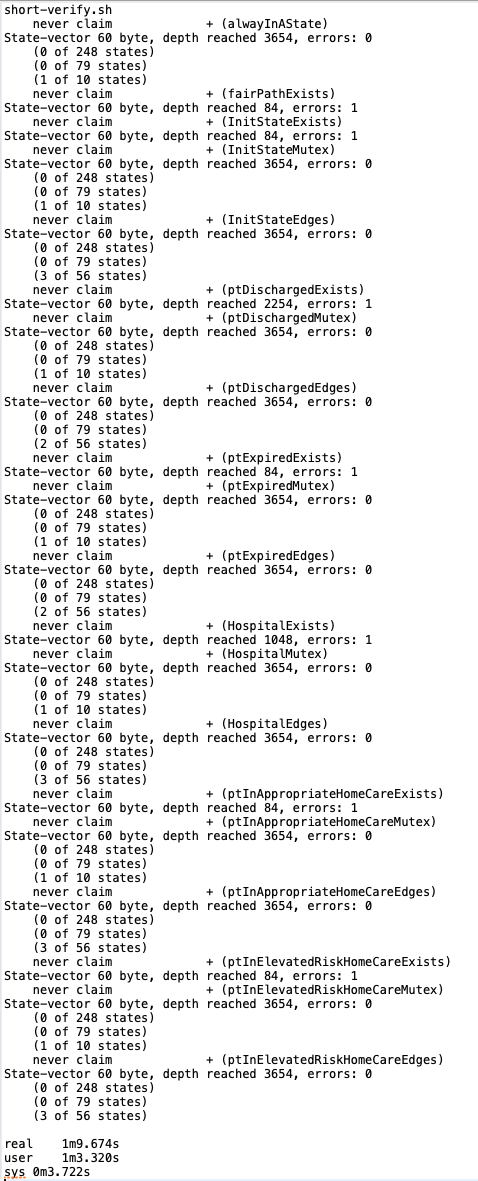
\includegraphics[scale=0.5]{proof.png}
    \end{tabular}
  \end{center}
\caption{The verification results from the SPIN model checker.}
\label{fig:proof}
\end{figure}

Verification takes around three to four minutes on an Intel Core i7 laptop with 16 Gb of RAM. It is not taxing the system in any way. The output from the script is shown in \figref{fig:proof}. The output names the property being verified (e.g., the \emph{never claim}). Following the named property, there is a  summary of the verification effort and what was proved. The critical value being the reported errors.

All the existential properties (i.e., the properties ending with \emph{Exists}) should result in an error. The error is the existential witness. All the other properties should pass with no errors. The output of the script includes not just the error report but the coverage summary of the processes and properties. The first two entries pertain to the clinician and patient-caregiver processes. There should never be uncovered states in these processes. Uncovered states means that there are unreachable behaviors in the model---not good. The third entry is the property being verified. It is not unusual to have uncovered states here when there is no reported error since the error behavior is not found in the model---good.

\section{Related Work}
There is some work related in translating models in the \emph{Business Process Execution Language} (BPEL) to Promela \cite{bpelToPromela}. BPEL semantics are different than BPMN semantics, and the work is limited in scope to modeling web-services. BPMN choreographies have been modeled in Promela and verified with SPIN for deadlock, but choreographies ignore workflows and only model message sequencing \cite{choreography}.

The translation of BPMN to Promela presented here is inspired by existing methods for turning Petri Nets into equivalent Promela models \cite{petrinetToPromela, petrinetInspiration}. These however do not include data as is needed to capture interactions with the CWP. The translation in this paper is also based off of early prototype translations of BPMN to Promela using message channels for synchronization \cite{bpmn2promela}. The translation in this paper uses global variables, and not message channels, for synchronization to mitigate state explosion.

\section{Conclusions and Future Work}
The CWP was coupled with workflow models to create a verification problem suitable for the SPIN model checker. This was accomplished by translating the CWP into an set of LTL properties that together express the same meaning as the CWP. The workflow models can be directly turned into equivalent models in Promela, the input language to SPIN, which is able to prove whether the workflows correctly implement the CWP. Such mechanized and automated reasoning is critical to assurance that the design of a complex distributed system is capable to establish and maintain \emph{actionable risk awareness}. 

The CWP defines thresholds of patient risk during home care and their appropriate actions, thereby making a clear connection from the verified design to its larger, societal purpose of safe care. Although the interaction between users and AI is only modestly complex, it strikes the balance needed to illustrate the full method with an example workflow that can be followed by readers without much BPMN familiarity. 
Once deployed, the complexity could easily increase if confirmation/dismissal of alerts is fed back to AI machine learning to increase alert accuracy.

Our approach's generality depends on discovery and modeling CWPs. Prior to model-checking CWPs their principles  were applied to human-computer integration for highly usable designs of integrated aircraft mission and maintenance scheduling \cite{workcentered}, joint U.S.-Russia maneuver planning for the \emph{International Space Station}  \cite{10.1145/1978942.1979311}, and health care coordination \cite{BERRY201615}. These CWPs define fundamental requirements for systems that must respond to events outside their direct control. The principles of CWP were recently adopted in the SysMl v.2 standard.

Model-checking scalability depends on workflows' number of asynchronous actors, synchronization points, etc. BPMN supports hierarchies of sub-processes for larger workflows, where CWPs may be defined for each; regardless, the case study is a key step towards automation. 

Our current research aims to automate CWP translation to LTL, and BPMN to Promela, so counter-examples from SPIN point directly to CWPs. This undertaking is a non-trivial engineering task as model checking requires domain expertise and the counter-examples produced by SPIN are infinite by virtue of LTL semantics. Ongoing efforts are refining the SPIN translations to include additional global states that correspond directly to CWP states and edges to simplify counter-example mapping. 

Other research under consideration could explore reuse of verified designs in watcher systems that monitor their deployed implementations. CWP models could also be used to derive efficiency measures, e.g., reducing the amount of activity that does not advance the CWP states could be a new approach to efficiency.  

The focus of conventional design methods is on software, which leaves important aspects of system success largely to chance. 
This paper's novel contribution is verifiable integration of human-computer teaming on cognitive tasks. 
The need is industry-wide. 
Expected benefits of verifiable integration include greater safety and reliability of systems for many other critical domains. 

ACKNOWLEDGEMENTS

Earlier parts of this research were funded by:
AHRQ#1R011HS021233-01A1, ONC-#1051059, and  AFRL #F33615-03-2-6315.

\bibliographystyle{IEEEtran}
{\small 
\bibliography{paper}}

\end{document}
